\chapter{Preliminarii}

\section{Alegerea tehnologiilor}

Procesul de dezvoltare a unei aplicații începe înaintea scrierii codului, când trebuie luate diverse decizii, precum tehnologiile ce urmează să fie folosite. Acestea decid performanța și nevoile viitoare de mententanță ale aplicației. În acest caz, tipul aplicației implică folosirea sa atât în contexte informale, cât și în contexte corporative, cu un flux de muncă monitorizat, ceea ce sugerează că utillizatorul normal va vizualiza înterfața pe un desktop, pe calculatorul pe care își desfășoară activitățile zilnice. Astfel, este la îndemână ca aplicația să fie web, astfel ca orice utilizator să o poată accesa prin intermediul unui browser. O variantă populară pentru structurarea unei astfel de aplicații este varianta client-server, unde front-end-ul este o aplicație de sine stătătoare, SPA(Single-page Application), și comunică prin call-uri API cu back-end-ul. Popularitatea celor două aspecte este susținută de statistici, raportul ecosistemului de dezvoltare software din 2023 întocmit de JetBrains pe baza a peste 26 000 de repondenți, stabilind site-urile web ca principala formă de software dezvoltată folosind Java\cite{java-ecosystem} și tehnologiile pentru construirea de Single Page Applications ca principalul context al utilizării JavaScript\cite{javascript-ecosystem}.

\subsection{Typescript\&React}
O aplicație MVC(Model-View-Controller) clasică întoarce prin end-point-urile ei View-uri, adică pagini HTML care urmează să fie afișate de browser. Prin urmare, fiecare navigare presupune pentru utilizator o nouă cerere, o așteptare pentru aducerea paginii și timp în plus pentru reîncărcarea DOM-ului. Pentru a minimiza aceste cereri, un dezvoltator se poate folosi de jQuery, dar acest proces este anevoios și implică mult cod. Din fericire, această abordare a devenit ineficientă o dată cu popularizarea conceptului de SPA. Un SPA trimite un singur fișier HTML, impreună cu multe instrucțiuni JavaScript pentru a evita aceste probleme. Cu atât mai mult, tehnologiile actuale, precum React, propun și un mod mai puțin anevoios de dezvoltare a componentei front-end.

Biblioteca React aduce o perspectivă structurată dezvoltării interfeței, prin definirea de componente reutilizabile în cadrul aplicație. Se poate păstra conceptul de rute și pagini cu ajutorul ReactRouter, pentru ca utilizarea în cadrul browserului să rămână fluidă, iar acestea vor fi în continuare generate dinamic. React este bazat pe scrierea de componente în JavaScript sau TypeScript, la alegerea dezvoltatorului. Filele .jsx sau .tsx vor fi transformate de transpiler într-un bundle care poate fi înțeles de către browser\cite{the_road_to_react}. Prin utilizarea unui DOM virtual, manipularea DOM-ului devine minimală iar aplicația răspunde rapid nevoilor de actualizare continuă a conținutului.

Utilizarea limbajului Typescript, în defavoarea limbajului JavaScript, este explicată prin minimizarea erorilor cauzate de inconsistența adusă de faptul ca JavaScript este un limbaj „loosely typed” („dinamically typed”) și de incertitudinea adusă de acest fapt. Astfel, prezența interfețelor și tipurilor de date bine stabilite facilitează dezvoltarea rapidă și stabilă. O parte din componentele UI sunt utilizate din biblioteca Ant Design, folositoare prin aspectul vizual unitar și formal, acompaniat de o documentație bine pusă la punct.

 \begin{figure}[H]
	\centering
 	 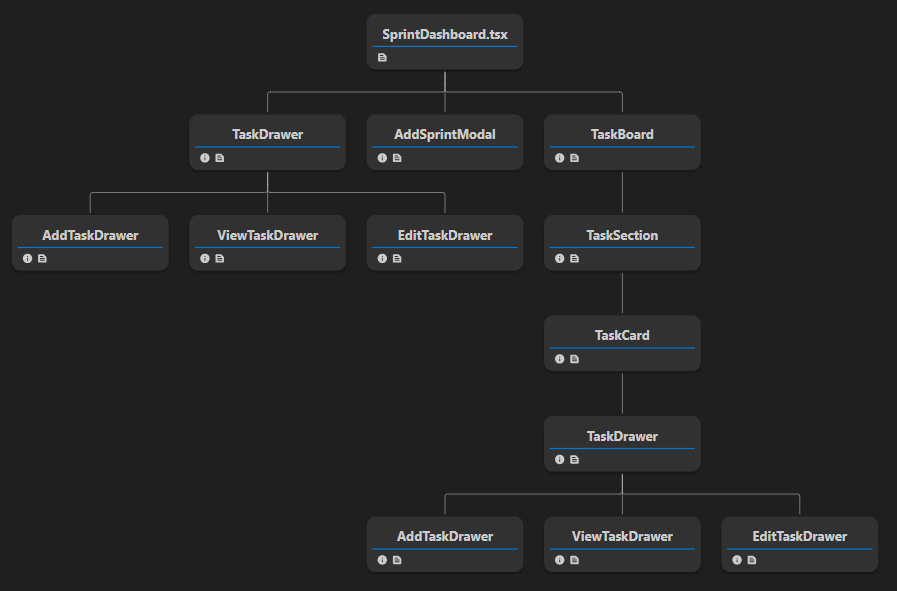
\includegraphics[width=\linewidth]{react-tree.png}
	\caption{Structura arborescentă a componentei Sprint Dashboard}
	\label{fig:react-tree}
 \end{figure}

Un aspect important al abordării prin componente este comunicarea între acestea, care devine greoaie atunci când complexitatea arborelui ierarhic crește. Un astfel de exemplu este pagina SprintDashboard, a cărei structură arborescentă este ilustrată în figura \ref{fig:react-tree}. Dacă, într-un astfel de context, am vrea să accesăm aceleași date în componente îndepărtate, precum TaskCard and EditTaskDrawer, ar trebui construit un sistem complex de props. Din acest motiv, orice aplicație React care urmărește o dezvoltare stabilă are nevoie de un state-manager, cele mai populare opțiuni fiind Redux și MobX. Dintre acestea, am ales MobX pentru abordarea lui bazată pe observers, un pattern ușor de înțeles, folosit într-o variantă mai complexă și de către framework-ul Angular. Acesta permite stocarea datelor necesare în zone necorelate ale aplicației într-un unic obiect și ușor accesibil.

\subsection{Java\&Spring}

Pentru partea de back-end a aplicației web am optat pentru limbajul Java și framework-ul Spring și ecosistemul acestuia, având în vedere opțiunile robuste pentru gestionarea logicii de afaceri, a securității și a interacțiunilor cu baza de date.\cite{why-spring}. Încadrarea Java în categoria limbajelor orientate pe obiect ajută la scrierea codului într-o manieră modulară, ușor de dezvoltat, dar și de menținut, având în vedere proprietatea centrală de compatibilitate retroactivă. Versiunea de Java utilizată este Java 21, cea mai recentă versiune de Java la momentul dezvoltării, pentru a avea acces la cele mai noi funcționalități,  precum noul garbage collector, esențial unui limbaj unde alocarea memoriei nu este gestionată de programator, care a primit update-uri de eficiență.

Versiunea de Spring folosită este 6.1.3, ce vine împreună cu Spring Boot 3.2.2, alături de alte dependințe, printre cele mai notabile numărându-se Spring Security și Jakarta Persistence API (JPA). Spring Boot simplifică procesul de dezvoltare prin punerea la dispoziție a unor funcționalități gata de utilizare, precum ar fi o serie de configurări și un sistem robust de injectare a dependințelor. Împreună cu biblioteca Lombok, acesta reduce semnificativ codul repetitiv, standard, accelerând procesul de dezvoltare.

Spring Cloud Gateway este o componentă care servește la crearea unui entry-point unic pentru cererile API-urilor. Aceasta este esențială într-o arhitectură bazată pe microservicii. Prin decuplarea aplicației client de serviciile de back-end, microserviciile se pot dezvolta și intergra în mod independent.

Pentru persistența datelor am ales PostgreSQL, un sistem open-source de gestiune pentru baze de date, pentru sistemul său de asigurare a integrității datelor și abilitatea de a manevra ușor cantități mari de date. Interacțiunea cu baza de date se face prin Spring Data JPA, care oferă o abstractizare la nivel înalt a stratului de persistență. În continuare, aceasta reduce codul repetitiv și suportă cereri complexe asupra bazei de date, codul sursă rămânând ușor de citit și înțeles.

O altă caracteristică importantă este securitatea, pentru care Spring Security oferă diverse opțiuni actuale de autentificare și autorizare, asigurând că aplicația se ridică la standardere și bunele practici curente.

\subsection{Python\&Flask}

Pentru microserviciul care se ocupă cu analiza datelor am ales Python, datorită opțiunilor variate de pachete și framework-uri pentru analiza și procesarea datelor. Mai exact, am folosit librăriile scikit-learn, pentru posibilitățile sale de data analysis și numpy, pentru capacitatea sa de computație numerică. Pentru interacțiunea cu aplicația am folosit framework-ul Flask, o alegere eficientă din punct de vedere a resurselor, potrivită unei aplicații ajutătoare. Abordarea sa minimalistă asigură o integrare ușoară cu restul sistemului. De asemenea, include un ORM pentru interacțiunea cu baza de date, SQLAlchemy. Acest ORM mapează și abstractizează simplu operațiile de citire de care am avut nevoie în această zonă a aplicației.

\section{Analiza și proiectarea aplicației}

\subsection{Actori}
Definirea funcționalităților principale este esențială pentru asigurarea îndeplinirii nevoii utilizatorilor. Aceasta implică identificarea tipurilor de utilizatori care vor interacționa cu aplicația și ce ar dori fiecare dintre ei. Analizând nevoile persoanelor care ar beneficia de acest gen de aplicație, principalii actori ai cazurilor de utilizare, identificați pe baza nevoilor specifice, sunt: 

- simplu membru de echipă: responsabil pentru îndeplinirea sarcinilor în timpul dat la dispoziție și pentru sincronizarea cu restul echipei

- manager al unei echipe: responsabil pentru gestionarea resurselor(și, în consecință, de atribuirea sarcinilor), urmărirea și analiza progresului proiectului

- administrator al platformei: responsabil de controlul și buna utilizare a platformei

\subsection{Identificarea cerințelor}
Pornind de la obiective, am creat o listă de cerințe pe care sistemul ar trebui să le indeplinească:

- sistemul trebuie să fie ușor de utilizat și să faciliteze management-ul proiectelor

- utilizatorii trebuie să se poată autentifica

- utilizatori cu roluri diferite trebuie să aibă niveluri de permisiune diferite

- să se poată crea, actualiza și șterge sarcini de lucru

- să se poată asigna sarcini de lucru pe baza performanțelor anterioare și a capacității

- să se poată verifica capacitatea membrilor echipei

- utilizatorii să fie notificați atunci când li se atribuie taskuri

- actualizări în timp real ale datelor

- generare de raporturi despre distribuția sarcinilor de lucru și performanța utilizatorilor

- interfață prietenoasă, accesibilă prin browser web, reactivă

- parolele trebuie să fie criptate înainte de salvarea în baza de date

- informațiile trebuie să fie protejate de eventuale atacuri, fiind confidențiale organizației

- sistemul trebuie să fie scalabil pentru a acomoda cerințe noi pe o piață dinamică

\subsection{Cazuri uzuale de utilizare}
Pe baza celor trei roluri și a cerințelor formulate, am izolat necesitățile funcționale și am listat câteva cazuri uzuale de utilizare, pentru a contura viitoarea aplicație din punct de vedere comportamental. Administatorul va primi autorizarea pentru activități de gestionare a platformei, managerul va avea nevoie de funcționalități cu ajutorul cărora să își gestioneze echipa, iar utilizatorul simplu, membru de echipă, va dispune de funcționalități pentru gestiunea propriului volum de muncă.

Funcționalitățile de bază pentru managerul de echipă sunt următoarele:

\begin{enumerate}
 	 \item În calitate de manager, aș vrea să adaug sarcini de lucru pentru echipa mea, cu detalii despre tipul sarcinii de lucru, criterii de acceptanță, prioritate, dificultate și termen limită pentru ca acestea să fie cât mai clare pentru membri echipei.

 	 \item În calitate de manager, aș vrea să creez sprinturi noi cu durată personalizată, pentru o delimitare bună a intervalelor de lucru.

 	 \item În calitate de manager, aș vrea să pot vizualiza factorii de performanță precum disponibilitatea, volumul de muncă, calificarea și atribuțiile fiecărui membru al echipei mele, pentru a evalua corect atribuirea de sarcini de lucru noi.

 	 \item În calitate de manager, aș vrea să atribui automat sarcini de lucru, bazat pe detaliile sarcinii de lucru și pe factorii de performanță angajatului, pentru a le împărți cât mai echitabil și a maximiza productivitatea și șansele ca sarcina să fie îndeplinită până la
termen.

 	 \item În calitate de manager, aș vrea să pot atribui manual sarcini de lucru, bazat pe analiza mea asupra situației, pentru a ajusta eventualele erori ale recomandărilor, a adapta panoul la noi informații relative la disponibilitate, sau a încuraja creșterea/scăderea productivității pentru un anumit membru al echipei.
\end{enumerate}

Pentru un membru obișnuit de echipă, cele mai de ajutor funcționalități sunt:
\begin{enumerate}
 	 \item În calitate de angajat obișnuit, aș vrea să îmi vizualizez sarcinile de lucru împreuna cu detalii despre tipul sarcinii de lucru, criterii de acceptanță, prioritate, dificultate și termen limită, pentru a îmi putea organiza activitatea zilnică.

 	 \item În calitate de angajat obișnuit, aș vrea să pot actualiza statusul sarcinilor de lucru pentru ca managerul meu să le cunoască progresul.

 	 \item În calitate de angajat obișnuit, aș vrea să fiu notificat atunci când managerul îmi atribuie o sarcina de lucru nouă, pentru a percepe mai ușor schimbări ale panoului cu sarcinile mele.

 	 \item În calitate de angajat obișnuit, aș vrea să văd în timp real actualizări ale panoului de lucru al echipei mele, pentru a fi mereu la curent cu statusul proiectului.

 	\item În calitate de angajat obișnuit, aș vrea să văd statistici ale performanței mele, pentru a mă putea auto-evalua.
\end{enumerate}

Un administator al platformei ar trebui să poată controla activitatea pe platformă în următoarele aspecte:
\begin{enumerate}
 	 \item  În calitate de administrator, aș vrea să pot crea, actualiza sau elimina utilizatori și echipe, pentru a putea gestiona accesul la platformă și organizarea internă.

 	 \item În calitate de administrator, aș vrea să pot atribui manageri echipelor create, pentru ca fiecare echipă să fie gestionată de un manager.

 	\item În calitate de administrator, aș vrea să pot verifica acțiunile făcute de utilizatori de platformă pentru a identifica eventuale erori.
\end{enumerate}

O practică comună în procesul de dezvoltare software este crearea de tabele de specificații care să descrie cazurile de utilizare, pentru o documentare clară a cerințelor stakeholder-ilor. În plus, într-un context real, acestea aliniază echipa de dezvoltare cu scopul urmărit, funcționând ca „single source of truth”. Pe baza cazului cu indicele 4 din setul utilizatorului de tip manager, am realizat tabelul din figura  \ref{fig:usecase-table}.

\begin{figure}[H]
	\centering
\begin{tabularx}{\textwidth} { 
  | >{\raggedright\arraybackslash}p{0.3\textwidth}
  | >{\raggedright\arraybackslash}p{0.7\textwidth} | }

 \hline
Nume &  Asignează automat sarcina de lucru\\
 \hline
Actor &  Manager \\
\hline
Descriere &  Permite oricărui manager să asigneze automat o sarcină de lucru unui membru al proriei echipe \\
\hline
Prioritate &  Funcționalitate de bază \\
\hline
Pre-condiții & - utilizatorul are un browser instalat pe dispozitiv și o conexiune stabilă la internet

- utilizatorul este autentificat cu un cont de tip manager

- există în baza de date cel puțin o sarcina de lucru anterioară  \\
\hline
Post-condiții & - noua sarcină de lucru este salvată în baza de date și poate fi vizualizată pe panou \\
\hline
Flux de bază & 1. Utilizatorul accesează Sprint Dashboard.

2. Utilizatorul deschide formularul de creare de nou task.

3. Utilizatorul completează câmpurile cu tipul de task, punctele de efort, prioritatea și sprintul.

4. a. Utilizatorul apasă butonul „Find best assignee”.

5. Utilizatorul primește o sugestie legat de asignare și o poate vizualiza.

6. a. Utilizatorul acceptă suggestia.

7. Utilizatorul salvează sarcina de lucru.\\
\hline
Fluxuri alternative & 6. b. Utilizatorul nu acceptă sugestia, caz în care trebuie să aleagă manual un membru al echipei.\\
\hline
Reguli business & - câmpurile cu tipul de task, punctele de efort, prioritatea și sprintul sunt obligatorii pentru cererea unei sugestii

- titlul, descrierea, estimarea în ore sunt obligatorii înainte de cererea de salvare a sarcinii de lucru\\
\hline
Cerințe non-funcționale & - integritatea datelor este necesară la salvarea în baza de date

- identitatea persoanei care încearcă să salveze datele trebuie să fie cunoscută\\
\hline
\end{tabularx}
	\caption{Specificațiile unui caz de utilizare}
	\label{fig:usecase-table}
\end{figure}